\chapter{Results}
\lhead{\emph{Results}}

\section{Scientific results}
This section will contain data, visualizations and results from the work associated with the scientific problem described in section \ref{problem_definition}.

In order to evaluate the different ANN models against each other, each model classified three different datasets in every iteration. Every training session therefore includes three different accuracy's, where each accuracy is calculated as correct predictions divided by total predictions.

The first dataset is the training set. This dataset consists of a large subset of data gathered from the CHROME dataset (90\%), and is the data the models used as training data. This dataset is labelled as \textit{train} in the accuracy graphs below. % små avsnitt? evt slå sammen?

The second dataset is the validation set, also called the test set. This dataset consists of the last 10\% of data from the CHROME dataset. None of the data in the validation set was used during training, and this data is therefore a good representation for how the model performs on unseen data. This dataset is labelled as \textit{test} in the accuracy graphs below.

The third dataset is a set of real data gathered from the example website, with symbols written by three different people. This dataset is used to give an indication of the correctness of the preprocessing, as well as how the model responds to data from different sources. The real dataset was an important inclusion because the main goal of this assignment was to produce good results under circumstances simulated by the example website. Notice that this dataset included a few mislabelled data points, contained only about three hundred data points, and includes only a subset of all the classes. The dataset is therefore only used as an indication of the accuracy on real data. This dataset is labelled as \textit{real} in the accuracy graphs below.

%TODO her må vi forklare hva train test og real er.
\begin{figure}[H]
    \centering
    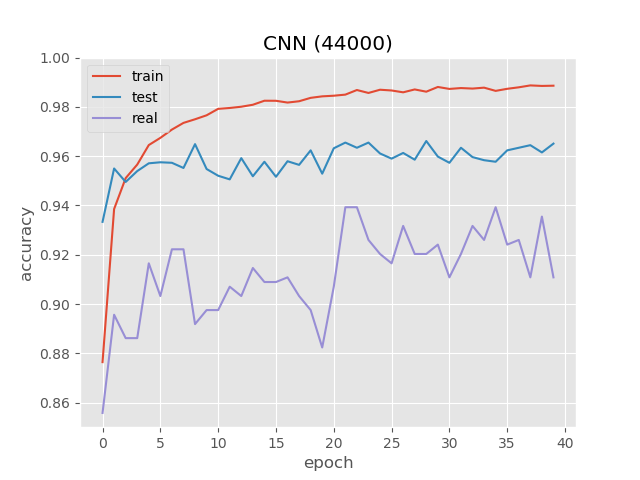
\includegraphics[width=0.8\linewidth]{Assets/Chapter4_Result/CNN_40_epoch.png}
    \caption{Training accuracy from the CNN model with 44000 data points evaluated for 40 epochs.}
    \label{fig:CNN_44000}
\end{figure}
\begin{figure}[H]
    \centering
    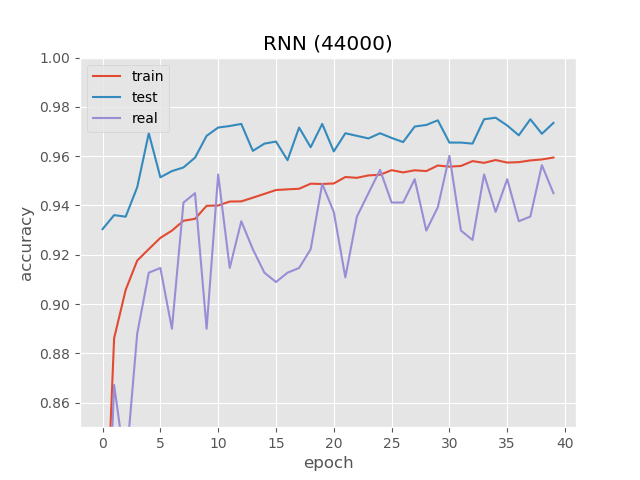
\includegraphics[width=0.8\linewidth]{Assets/Chapter4_Result/RNN_40_epoch.png}
    \caption{Training accguracy from the RNN model with 44000 data points evaluated for 40 epochs.}
    \label{fig:RNN_44000}
\end{figure}

\begin{figure}[H]
    \centering
    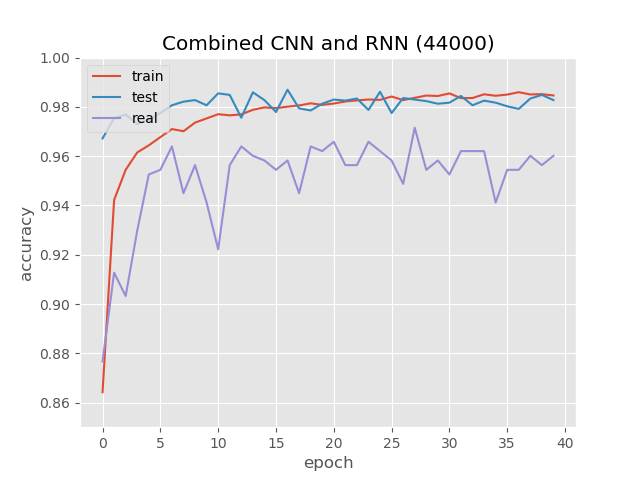
\includegraphics[width=.8\linewidth]{Assets/Chapter4_Result/Combined_CNN_and_RNN_40_epoch.png}
    \caption{Training accuracy from the combined CNN and RNN model with 44000 datapoints. Evaluated for 40 epochs.}
    \label{fig:combined_CNN_RNN_44000}
\end{figure}

The tables below show the same data in tabular form. Each row is a snapshot of the different models' accuracy in percent at specific epochs. 

Table of the \textbf{train} dataset.
\begin{figure}[H]
    \centering
        \begin{tabular}{| p{2cm} | p{3cm} | p{3cm} | p{3cm} |}
    \hline
    Epoch & \textbf{CNN} & \textbf{RNN} & \textbf{Combined} \\ \hline
    10 & 97.66 & 93.99 & 97.53 \\ \hline
    20 & 98.43 & 94.87 & 98.08 \\ \hline
    30 & 98.81 & 95.62 & 98.44 \\ \hline
    40 & 98.86 & 95.95 & 98.46 \\ \hline
    \end{tabular}
    \caption{Snapshot of accuracy in percent on the train dataset for all models at epoch number 10, 20, 30 and 40}

    \label{fig:table_train_dataset}
\end{figure}

Table of the \textbf{test} dataset.
\begin{figure}[H]
    \centering
    \begin{tabular}{| p{2cm} | p{3cm} | p{3cm} | p{3cm} |}
    \hline
    Epoch & \textbf{CNN} & \textbf{RNN} & \textbf{Combined} \\ \hline
    10 & 95.48 & 96.82 & 98.07 \\ \hline
    20 & 95.29 & 97.31 & 98.13 \\ \hline
    30 & 95.98 & 97.46 & 98.13 \\ \hline
    40 & 96.51 & 97.35 & 98.28 \\ \hline
    \end{tabular}
    \caption{Snapshot of accuracy in percent on the test dataset for all models at epoch number 10, 20, 30 and 40}
    \label{fig:table_test_dataset}

\end{figure}

Table of the \textbf{real} dataset.
\begin{figure}[H]
    \centering
    \begin{tabular}{| p{2cm} | p{3cm} | p{3cm} | p{3cm} |}
    \hline
    Epoch & \textbf{CNN} & \textbf{RNN} & \textbf{Combined} \\ \hline
    10 & 89.75 & 88.99 & 94.12 \\ \hline
    20 & 88.24 & 94.88 & 96.20 \\ \hline
    30 & 92.41 & 93.93 & 95.83 \\ \hline
    40 & 91.08 & 94.50 & 96.02 \\ \hline
    \end{tabular}
    \caption{Snapshot of accuracy in percent on the real dataset for all models at epoch number 10, 20, 30 and 40}
    \label{fig:table_real_dataset}

\end{figure}

\section{Engineering results}
This section will contain how our example project/proof of concept has turned out in terms of goals set in earlier stages of the project. The evaluation of engineering result is based on goals set in meetings with the product owners. % Resultat fra tester skal være lagt her

The product was intended to be a proof of concept application, with functionality for recognizing handwritten mathematical symbols. In addition, it was meant to be used as a module to enhance Matistikk's functionality. Therefore, the product had to be easily integrable to the already existing Matistikk. 


\begin{figure}[H]
    \centering
    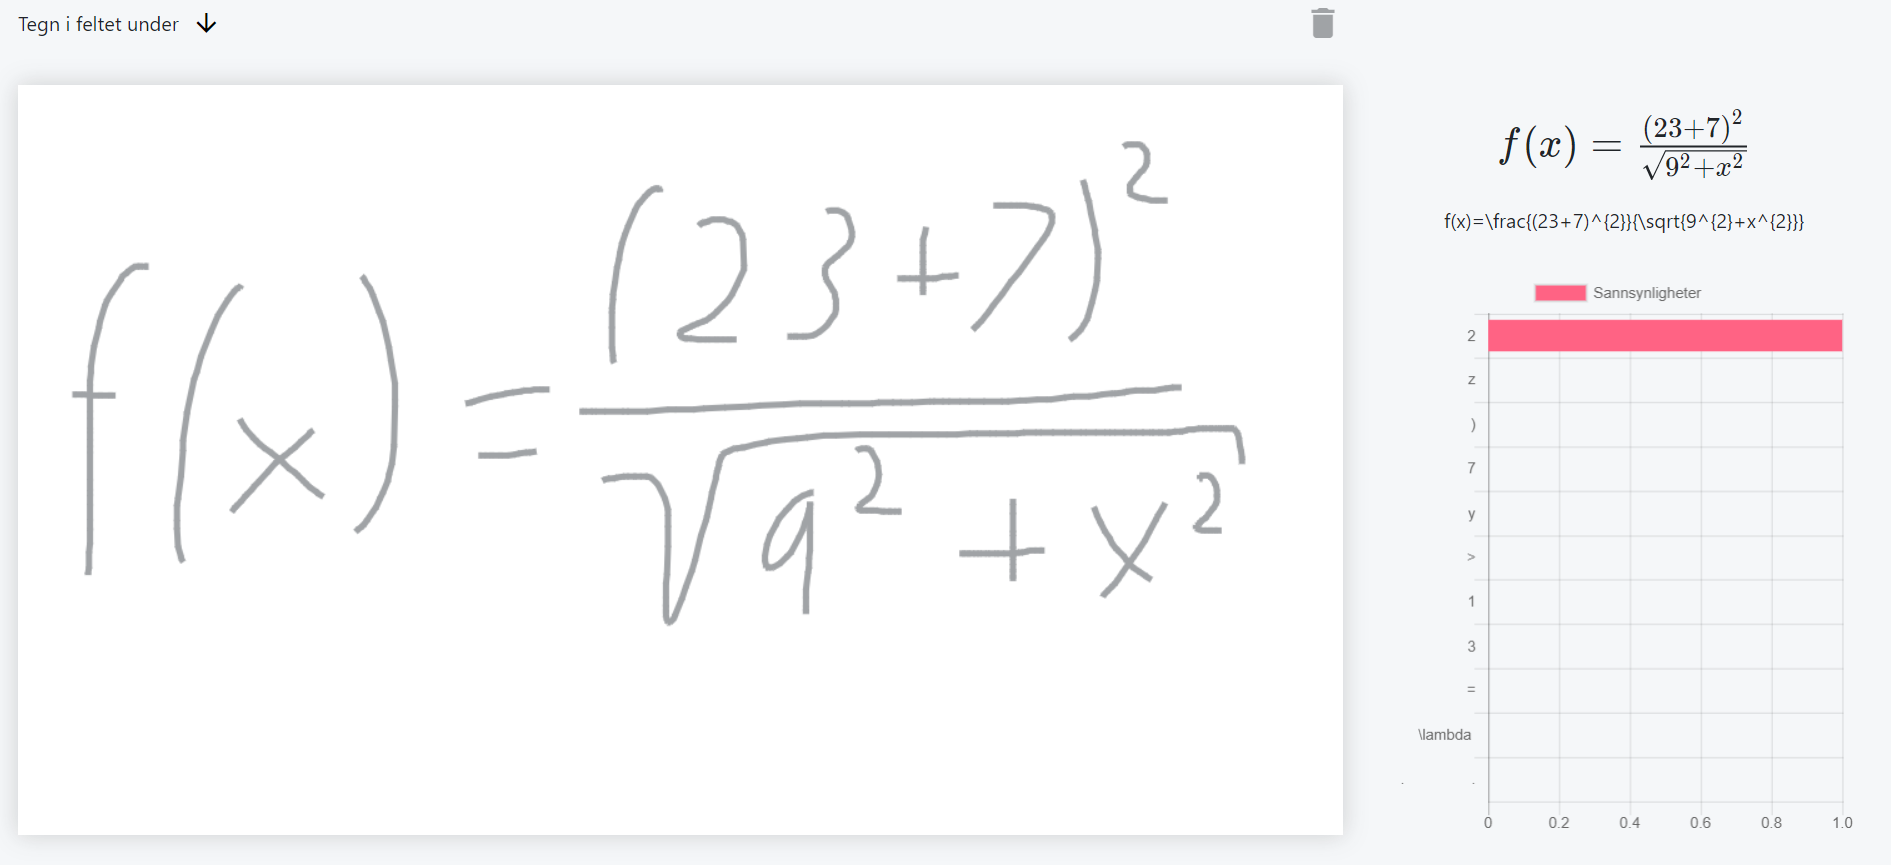
\includegraphics[width=\textwidth]{Assets/Chapter4_Result/predictor_example.png}
    \caption{Example of the graphical user interface, with an HTML5 canvas. The result is shown at the top right corner in human readable form. Directly below is the corresponding \LaTeX script, which can be useful for further use in other APIs. The graph on the right contains the classification probabilities for either a chosen symbol or the latest drawn.}
    \label{fig:predictor_example}
\end{figure}

The back- and front end is developed as two separate products. These can be integrated independently into a larger system. An example implementation of this is deployed on Heroku, a cloud application platform.

Results from the algorithms behind segmentation and context was not easily measurable. They are however discussed in chapter \ref{engineering_results}.

\section{Administrative results}
Administrative results is the results of planning, implementing, researching and concluding the work done in this project. 

Due to the high uncertainty in the assignment, the planning had to be done in a dynamic process continuously through the project. After each small period it was necessary to do a retrospective, to learn from mistakes and further improve the project flow and productivity. Incorporating iterations and reviews into the project flow enhanced the ability to respond to changes and new goals. Modern Agile principles were followed during the project, and was a good fit for a research based assignment. Detailed planning was achievable when developing the foundation of the web-based system. 
